\documentclass[../main.tex]{subfiles}
\graphicspath{{\subfix{../images/}}}


\begin{document}
Python
\subsection{Libraries used}

Keras

Tensorflow (GPU)

Pandas

Numpy

Geopandas

Packages and programming language used.


\subsection{Data pre processing}

What range of data was used for the final model and reason for so. The problems with AIS data and getting clean routes from start to finish and primarily enough routes for training and testing. 

Processing the HELCOM data to extract routes that can be used to train a model with the goal in mind.


\subsubsection{Algorithm for extracting routes from dataset}

Explain the algorithm behind getting the routes from the raw data set and that the idea can be applied to any port or area of interest really by defining the area of interest.

The largest gaps allowed

The port chosen for the evaluation has its caveats and should perhaps be identified.

Validation of the routes extracted i.e gaps, no shorter than n number of messages where the vessel is going, not returning to port, longer than n hours, no faulty data etc.

\begin{figure}[H]
	\centering
	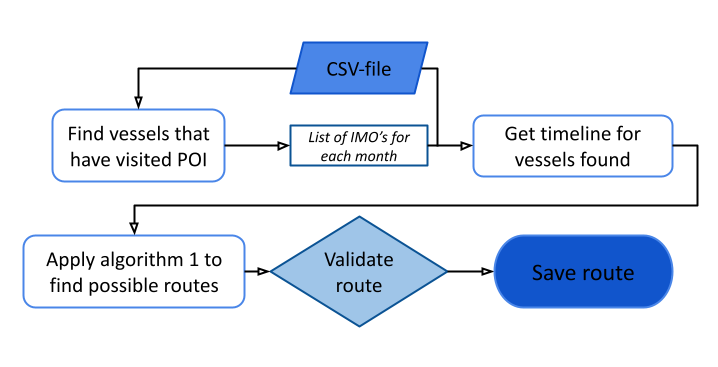
\includegraphics[scale=.5]{data-process(2).png}
	\caption{Getting routes.}
	\label{fig:flowchart}
\end{figure}

POI (port of interest could also be thought of as Area of Interest). Timeline is the vessels historical data which is fed into algorithm 1. Route validation according to rules and then save the complete route.

\subsubsection{Coordinate accuracy}

Scaling the accuracy from raw data to a suitable accuracy. GIS decimal degrees

Vessel travelling at 14 knots (25 km/h) and a message interval of 10 minutes approx. will move 2.2 nmi (4.1 km) per message


\subsubsection{Feature selection}

The features chosen for the final training 

Latitude, longitude, sog, cog, vessel class, draught, ?distance? 

The target is Time To Destination, how many minutes are left to the destination


\subsubsection{Time series data preparation and cleanliness}

Further details on how the processed routes are handled to generate the training data to utilize multiple timesteps per prediction which improves performance. Also why the number of timesteps per prediction was chosen, with the time normalized data and how many steps then per time window. 

The largest allowed difference between messages in the time normalized data

\subsection{ML model}

Description of the neural network model used and tested to find the optimal performer


\subsection{Comparison model}

!!! If the travel distance left to destination is used in nmi for example, test the accuracy against simply calculating time left by the current speed and distance left 

\end{document}